\begin{solution}
\begin{enumerate}
\item Follow the usual methodology:  Substitute the form
\[ u(x,t) = \sum_{n=1}^\infty a_n(t) \psi_n(x)\]
into the differential equation $u_{tt} = u_{xx} - 2d u_t$ to obtain
\begin{eqnarray*}
   \sum_{n=1}^\infty a''_n(t) \psi_n(x)
    &=& \sum_{n=1}^\infty a_n(t) \psi''_n(x)
    - 2 d \sum_{n=1}^\infty a'_n(t) \psi_n(x) \\[0.5em]
    &=& -\sum_{n=1}^\infty \lambda_n a_n(t) \psi_n(x)
    - 2 d \sum_{n=1}^\infty a'_n(t) \psi_n(x).
\end{eqnarray*}
Take the inner product with the eigenfunction $\psi_k$
and use orthogonality of the eigenfunctions to obtain
\[ a''_k(t) = -\lambda_k a_k(t) -2 d a'_k(t)\]
as required.
\item We first compute two derivatives of the proposed formula for $a_k$:
\begin{eqnarray*}
a_k'(t) &=& C_1 \big(-d + \sqrt{d^2 -k^2\pi^2}\big) 
                 \exp\!\big(\big(-\!d+\sqrt{d^2-k^2\pi^2}\big)t\big) \\[0.25em]
        & & {}+C_2 \big(-d - \sqrt{d^2 -k^2\pi^2}\big)
                 \exp\!\big(\big(-\!d-\sqrt{d^2-k^2\pi^2}\big)t\big) \\[1em]
a_k''(t) &=& C_1 \big(-d - \sqrt{d^2 -k^2\pi^2}\big)^2 
                 \exp\!\big(\big(-\!d+\sqrt{d^2-k^2\pi^2}\big)t\big) \\[0.25em]
        & & {}+C_2 \big(-d + \sqrt{d^2 -k^2\pi^2}\big)^2
                 \exp\!\big(\big(-\!d-\sqrt{d^2-k^2\pi^2}\big)t\big).
\end{eqnarray*}
We wish to verify that $a_k''(t) = -\lambda_k a_k(t) - 2d a'_k(t)$,
where $\lambda_k = k^2\pi^2$.  We can see that
\begin{eqnarray*}
   -\lambda_k a_k(t) - 2d a'_k(t)
     &=& C_1\Big(-\lambda_k - 2d \big(-d + \sqrt{d^2 -k^2\pi^2}\big)\Big)
                \exp\!\big(\big(-\!d+\sqrt{d^2-k^2\pi^2}\big)t\big) \\[0.25em]
     &&{}+ C_2\Big(-\lambda_k - 2d \big(-d - \sqrt{d^2 -k^2\pi^2}\big)\Big)
                \exp\!\big(\big(-\!d-\sqrt{d^2-k^2\pi^2}\big)t\big) \\[1em]
     &=& C_1\big(-k^2\pi^2 + 2d^2 - 2d \sqrt{d^2 -k^2\pi^2}\big)
                \exp\!\big(\big(-\!d+\sqrt{d^2-k^2\pi^2}\big)t\big) \\[0.25em]
     &&{}+ C_2\big(-k^2\pi^2 + 2d^2 + 2d \sqrt{d^2 -k^2\pi^2}\big)
                \exp\!\big(\big(-\!d-\sqrt{d^2-k^2\pi^2}\big)t\big) \\[1em]
     &=& C_1\big(-d+\sqrt{d^2 -k^2\pi^2}\big)^2
                \exp\!\big(\big(-\!d+\sqrt{d^2-k^2\pi^2}\big)t\big) \\[0.25em]
     &&{}+ C_2\big(-d-\sqrt{d^2 -k^2\pi^2}\big)^2
                \exp\!\big(\big(-\!d-\sqrt{d^2-k^2\pi^2}\big)t\big).
\end{eqnarray*} 
This final formula agrees with the formula for $a''_k(t)$ we computed earlier,
and thus we have confirmed that this is a general solution for our differential equation.

\item We need to now compute $C_1$ and $C_2$ so that $a_k(0)=0$ and $a_k'(0)=b_k(0)$.
      At $t=0$, the general solution becomes
      \[ a_k(0) = C_1 \exp(0) + C_2 \eps(0) = C_1 + C_2,\]
      so $a_k(0) = 0$ requires that 
           \[ C_1 = -C_2. \]
      Taking the formula for $a_k'(t)$ in part~(b) and evaluating at $t=0$ gives
      \[ a_k'(0) = C_1 \big(-d + \sqrt{d^2 -k^2\pi^2}\big)
                    + C_2 \big(-d - \sqrt{d^2 -k^2\pi^2}\big).\]
      So with $C_1 = -C2$ and $a_k'(0) = b_k(0)$, we arrive at
       \[ C_1 = -C_2 = {b_k(0) \over 2 \sqrt{d^2- k^2\pi^2}}.\]

\item The requested solutions, varying in $t$ with fixed $d$,
      are collected in the plot below.
     
      \begin{center} 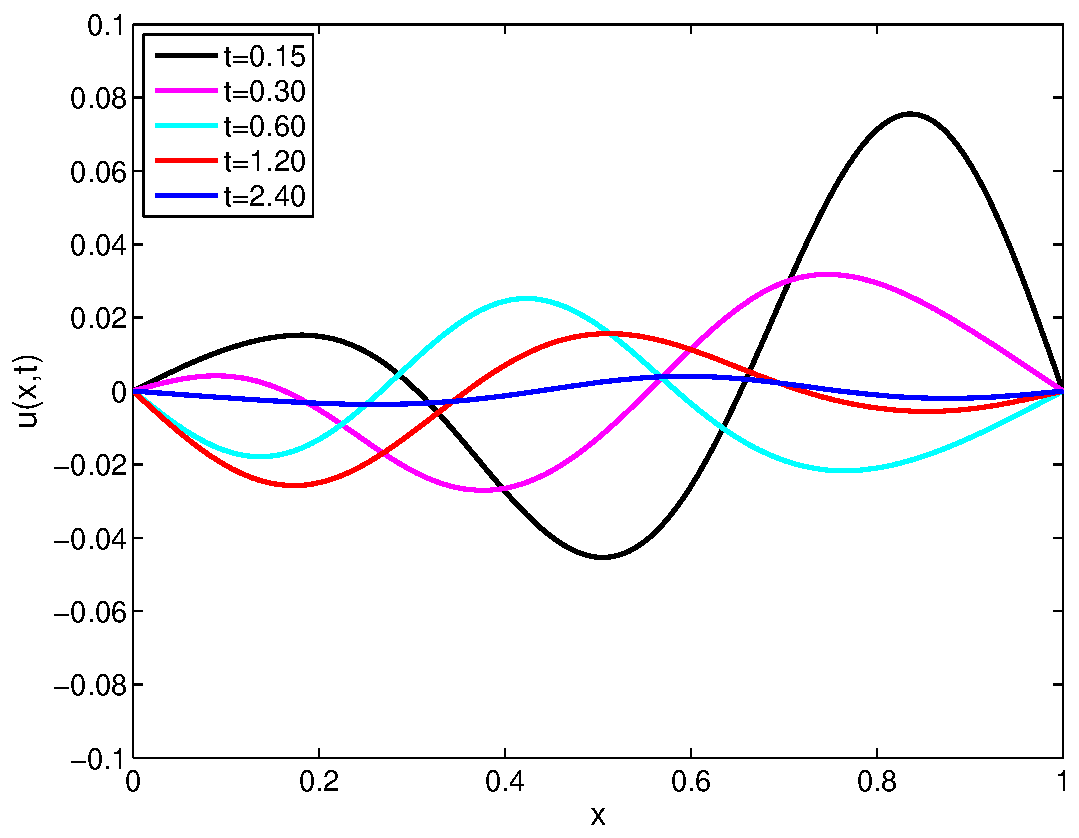
\includegraphics[scale=0.6]{damp1}\end{center}

{\small\begin{verbatim}
 tvec = [.15 .30 .60 1.20 2.40];
 xx = linspace(0,1,500)';

 ak0 = zeros(10,1);
 bk0 = zeros(10,1);
 k = [1:20]';
 bk0 = -6*sqrt(2)*(1+(-1).^k).*k./((k.^2-9).^2*pi^2);
 bk0(3) = sqrt(2)/4;

 d = 1;

 col = 'kmcrb';
 figure(1), clf
 for m=1:length(tvec)
    t = tvec(m)
    u = zeros(size(xx));
    for k=1:length(bk0)
        psik = sqrt(2)*sin(k*pi*xx);
        dis = sqrt(d^2-k^2*pi^2);
        ak = bk0(k)*(exp((-d+dis)*t)-exp((-d-dis)*t))/(2*dis);
        u = u+ak*psik;
    end 
    plot(xx,u,'-','linewidth',2,'color',col(m)), hold on
    ylim([-.1 .1])
    pause
 end
 legend('t=0.15','t=0.30','t=0.60','t=1.20','t=2.40',2)
 set(gca,'fontsize',14)
 xlabel('x','fontsize',16)
 ylabel('u(x,t)','fontsize',16)
 print -depsc2 damp1.eps
\end{verbatim}}

\item The requested solutions, now varying in $d$ with fixed $t$,
      are collected in the plot below.  As the damping parameter 
      increases on $(0,\pi)$, the solution gets increasingly smaller
      in amplitude at this time.
     
      \begin{center} 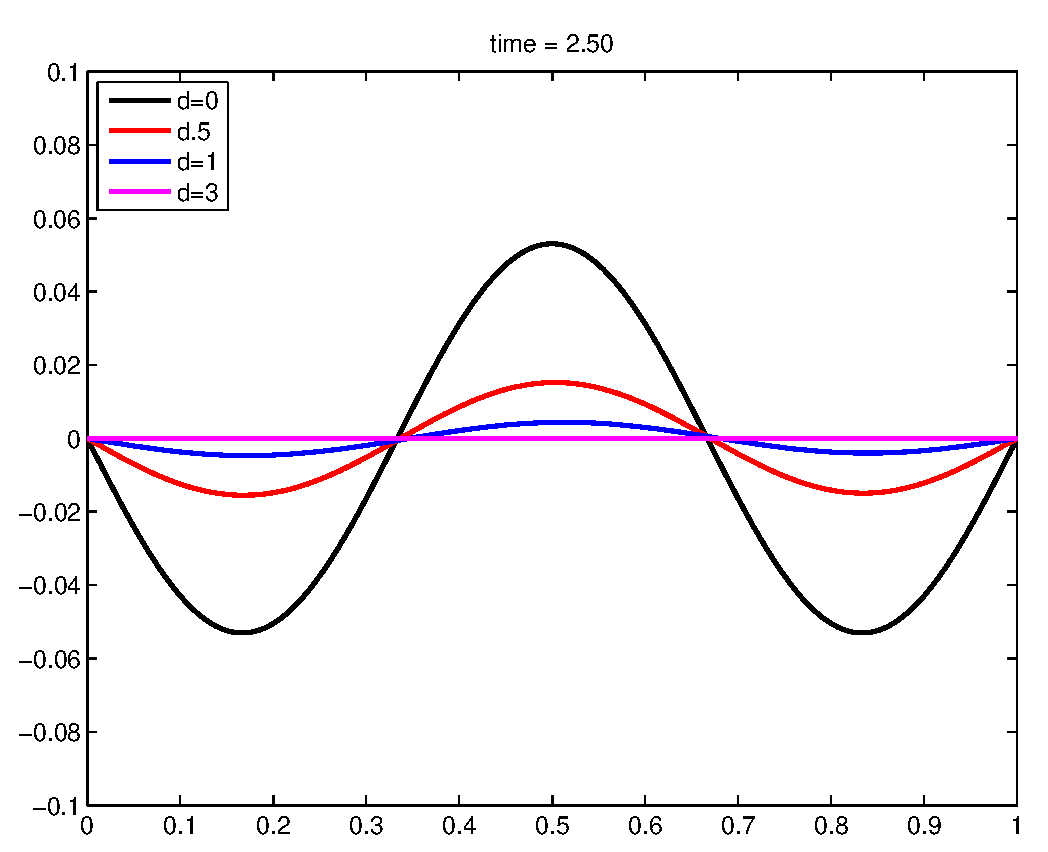
\includegraphics[scale=0.6]{damp2}\end{center}

{\small\begin{verbatim}
 t = 2.5;
 dvec = [0 .5 1 3];
 xx = linspace(0,1,500)';

 ak0 = zeros(10,1);
 bk0 = zeros(10,1);
 k = [1:20]';
 bk0 = -6*sqrt(2)*(1+(-1).^k).*k./((k.^2-9).^2*pi^2);
 bk0(3) = sqrt(2)/4;

 figure(1), clf
 cvec = 'krbm';
 for m=1:length(dvec)
    d = dvec(m)
    u = zeros(size(xx));
    for k=1:length(bk0)
        psik = sqrt(2)*sin(k*pi*xx);
        dis = sqrt(d^2-k^2*pi^2);
        ak = bk0(k)*(exp((-d+dis)*t)-exp((-d-dis)*t))/(2*dis);
        u = u+ak*psik;
    end 
    plot(xx,u,'-','linewidth',2,'color',cvec(m)), hold on
    ylim([-.1 .1])
    title(sprintf('time = %3.2f', t))
 end
 legend('d=0','d=.5','d=1','d=3',2)
 print -depsc2 damp2.eps
\end{verbatim}}

\end{enumerate}
\end{solution}
